\chapter{スタートプロジェクトの作成}
\label{chap:02-create-react-app}
\begin{starterabstract}
  この章では、「create{-}react{-}app」と言う、reactアプリケーションの雛形がコマンドひとつで作成できる優れものを使用して、
スタート用のアプリケーションを作成し、ブラウザで表示するまでを行います。

 また、作成するプロジェクトは、Typescriptを使用します。コード記法の指摘・修正を行えるよう「eslint」、「prettier」の設定も行います。

\end{starterabstract}

\section{create{-}react{-}appコマンド}
\keeplastskip{
  \label{sec:2-1}
  \label{sec-01command}
  \par\nobreak
}

Reactアプリケーションを作成するためには、

\begin{starteritemize}
\item 「nodeプロジェクト」に必要なpackage.jsonを作成
\item reactなど必要なライブラリのインストール
\item 作成したアプリケーションが、古いブラウザでも実行できるようにコードを変換(babel使用)
\item 出力するファイルを纏める(バンドルする{-}webpack使用)
\end{starteritemize}

など、reactライブラリのインストール以外にも、babelやwebpackをインストールして設定ファイルを作成し、
使用するライブラリーによっては、babelのプラグインのインストールや設定など、アプリケーションのコードを書き始める前の作業が大変です。

しかし、「そんなメンドウなことは、やってられない。」ので、
すぐにでもコードを書き始めることのできるスタート用アプリケーションが、reactの開発元であるFacebookから提供されています。

更に、そのスタート用アプリケーションは、コマンド一発でインストールすることができます。

ターミナルを起動し、プロジェクトフォルダを作成するフォルダへ移動します。

\def\startercodeblockfontsize{}
\begin{starterterminal}[]{create{-}react{-}appでスタート用アプリケーション作成}\seqsplit{  \textdollar{} \textgreater{} yarn create react{-}app プロジェクト名 {-}{-}template typescript}\end{starterterminal}

で、「プロジェクト名」のフォルダが作成され必要なライブラリがインストールされます。

\def\startercodeblockfontsize{}
\begin{starterterminal}[]{}\seqsplit{  Success! Created yourproject at /Users/tmkkz/Documents/Devs/playground/yourproject
  Inside that directory, you can run several commands:

    yarn start
      Starts the development server.

    yarn build
      Bundles the app into static files for production.

    yarn test
      Starts the test runner.

    yarn eject
      Removes this tool and copies build dependencies, configuration files
      and scripts into the app directory. If you do this, you can’t go back!

  We suggest that you begin by typing:

    cd yourproject
    yarn start

  Happy hacking!}\end{starterterminal}

で、プロジェクト作成が完了します。

\begin{starternote}[]{github}

ここまでの作業は、githubにあります。以下のコマンドでクローンしてください。

\def\startercodeblockfontsize{}
\begin{starterterminal}[]{githubから}\seqsplit{    \textdollar{} \textgreater{} git clone {-}b 00\textunderscore{}create{-}react{-}app https://github.com/tmkkz/yaruo.git}\end{starterterminal}
\end{starternote}

\section{アプリケーションを実行}
\keeplastskip{
  \label{sec:2-2}
  \label{sec-02yarnstart}
  \par\nobreak
}

アプリケーションが作成出来ましたので、実行してみます。

ターミナルに表示されているように、プロジェクトフォルダへ移動し、スタート用のコマンドを入力します。

\def\startercodeblockfontsize{}
\begin{starterterminal}[]{}\seqsplit{  \textdollar{} \textgreater{} cd プロジェクト名
  \textdollar{} \textgreater{} yarn start}\end{starterterminal}

すると、webpackに同梱されている開発用のweb serverが起動し、ディフォルトでは、port:3000でアプリケーションへアクセスできます。

\def\startercodeblockfontsize{}
\begin{starterterminal}[]{}\seqsplit{Compiled successfully!

You can now view yourproject in the browser.

  Local:            http://localhost:3000
  On Your Network:  http://192.168.1.10:3000

Note that the development build is not optimized.
To create a production build, use yarn build.}\end{starterterminal}

Google Chromeが起動し、http://localhost:3000へアクセスし以下のページが表示されます。

\begin{reviewimage}[H]%%02_cra_start
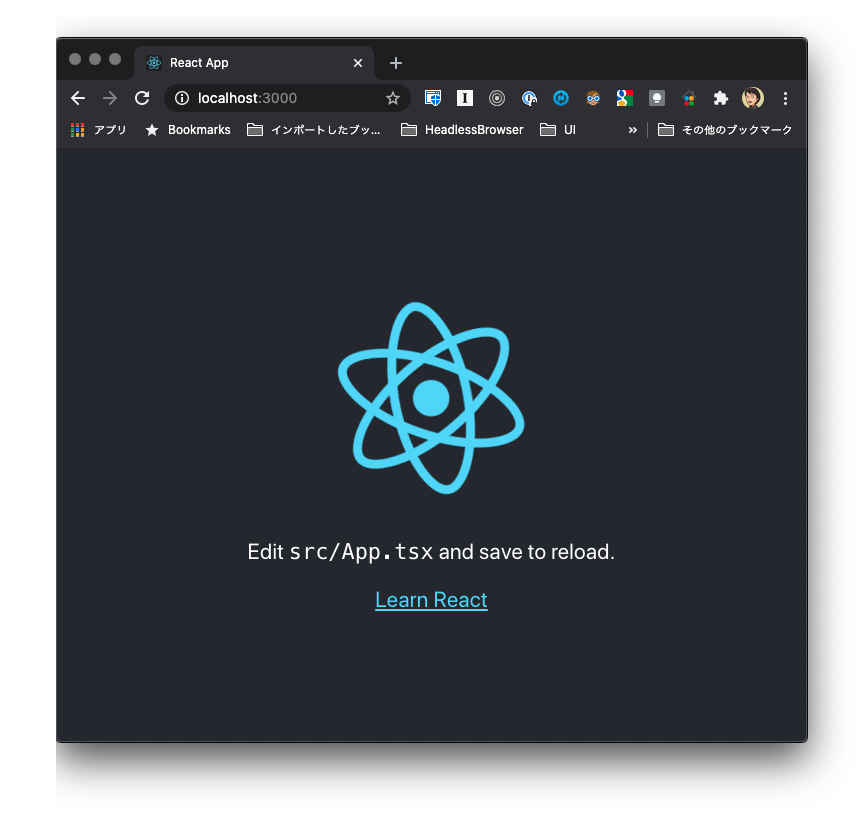
\includegraphics[width=1.0\maxwidth]{./images/02-create-react-app/02_cra_start.png}%
\reviewimagecaption{create{-}react{-}appの画面}
\label{image:02-create-react-app:02_cra_start}
\end{reviewimage}

このページが表示されれば成功です。

\section{eslint、prettierのインストールと設定}
\keeplastskip{
  \label{sec:2-3}
  \label{sec-03lint}
  \par\nobreak
}

あなたがプロジェクトチームに参加しているのであれば、そのチームのコーディング規約に沿うことが求められます。

例えば、

\begin{starteritemize}
\item ファイル、コンポーネント、関数などの命名規則
\item 文末のセミコロン
\item 改行位置
\end{starteritemize}

など、チーム毎、プロジェクト毎にコーディングがあります。

また、JavaScriptでは、「es5」などの標準仕様がありますので、どの標準仕様に沿ってコーディングするのかも指定されます。

自分ではコーディング規約に沿っているつもりでも、レビューを受けるまで知らなかったり、見落としていたりします。

そのため、コーディング規約に沿っているかを、

\begin{starteritemize}
\item 自動でチェック
\item 自動で修正
\item 修正方法の提案
\end{starteritemize}

などをしてくれる便利なものがありますので、積極的に使うようにしましょう。

この便利な機能こそが、第1章で紹介した

\begin{starteritemize}
\item Eslint
\item Prettier
\end{starteritemize}

になります。

しかし、残念ながらEslintもPrettierも

\begin{starteritemize}
\item 沢山のプラグインがある
\item EslintとPrettierが競合する部分もある
\end{starteritemize}

など、メンドウなことが沢山あります。

オープンソースの世界では、メンドウなことは大抵を先人が解決してくれている、もしくは、解決しようとしている最中です。
もし、解決しようとしている最中で出来ることがあれば手伝いたいものです。

この「Eslint、Prettier」のインストール・設定についても以下の方法で簡単に解決ができます。

eslint{-}config
\url{https://www.npmjs.com/package/@abhijithvijayan/eslint-config}

こちらは、自分で使われている「Eslint、Prettier」のプラグイン・設定を公開し、
コマンド一発でインストール完了すうるようにしてくれています。

\def\startercodeblockfontsize{}
\begin{starterterminal}[]{コマンド一発でインストール}\seqsplit{  \textdollar{} \textgreater{} npx install{-}peerdeps @abhijithvijayan/eslint{-}config {-}{-}dev {-}{-}yarn}\end{starterterminal}

このプロジェクトは、

\begin{starteritemize}
\item React
\item Typescript
\end{starteritemize}

を使っていますので、

プロジェクトのルートフォルダに、「.eslintrc.json」ファイルを作成し、以下のように設定をしてください。

私の好みで、Prettierにて

\begin{starteritemize}
\item 必要な箇所には、セミコロンを付ける
\item 文字列は、ダブルクォートで囲む
\end{starteritemize}

と、しています。

それ以外では、airbnbを元に基本的なルールが設定してあります。ルールは、「.eslintrc.json」で上書きできますので
ご自分の好みで変更してください。

\def\startercodeblockfontsize{}
\begin{starterprogram}[]{.eslintrc.json}\seqsplit{  \{
    "extends": [
      "@abhijithvijayan/eslint{-}config/typescript",
      "@abhijithvijayan/eslint{-}config/react"
    ],
    "parserOptions": \{
      "project": "./tsconfig.json"
    \},
    "rules": \{
      "react/jsx{-}props{-}no{-}spreading": "off",
      "prettier/prettier": [
        "error",
        \{
          "semi": true,
          "singleQuote": false
        \}
      ]
    \}
  \}}\end{starterprogram}

Eslint、Prettierの設定が完了しましたので、srcフォルダにある「App.tsx」を開いてみると、
コーディング規約に外れるものは指摘されています。

\begin{reviewimage}[H]%%03_eslint_prettier
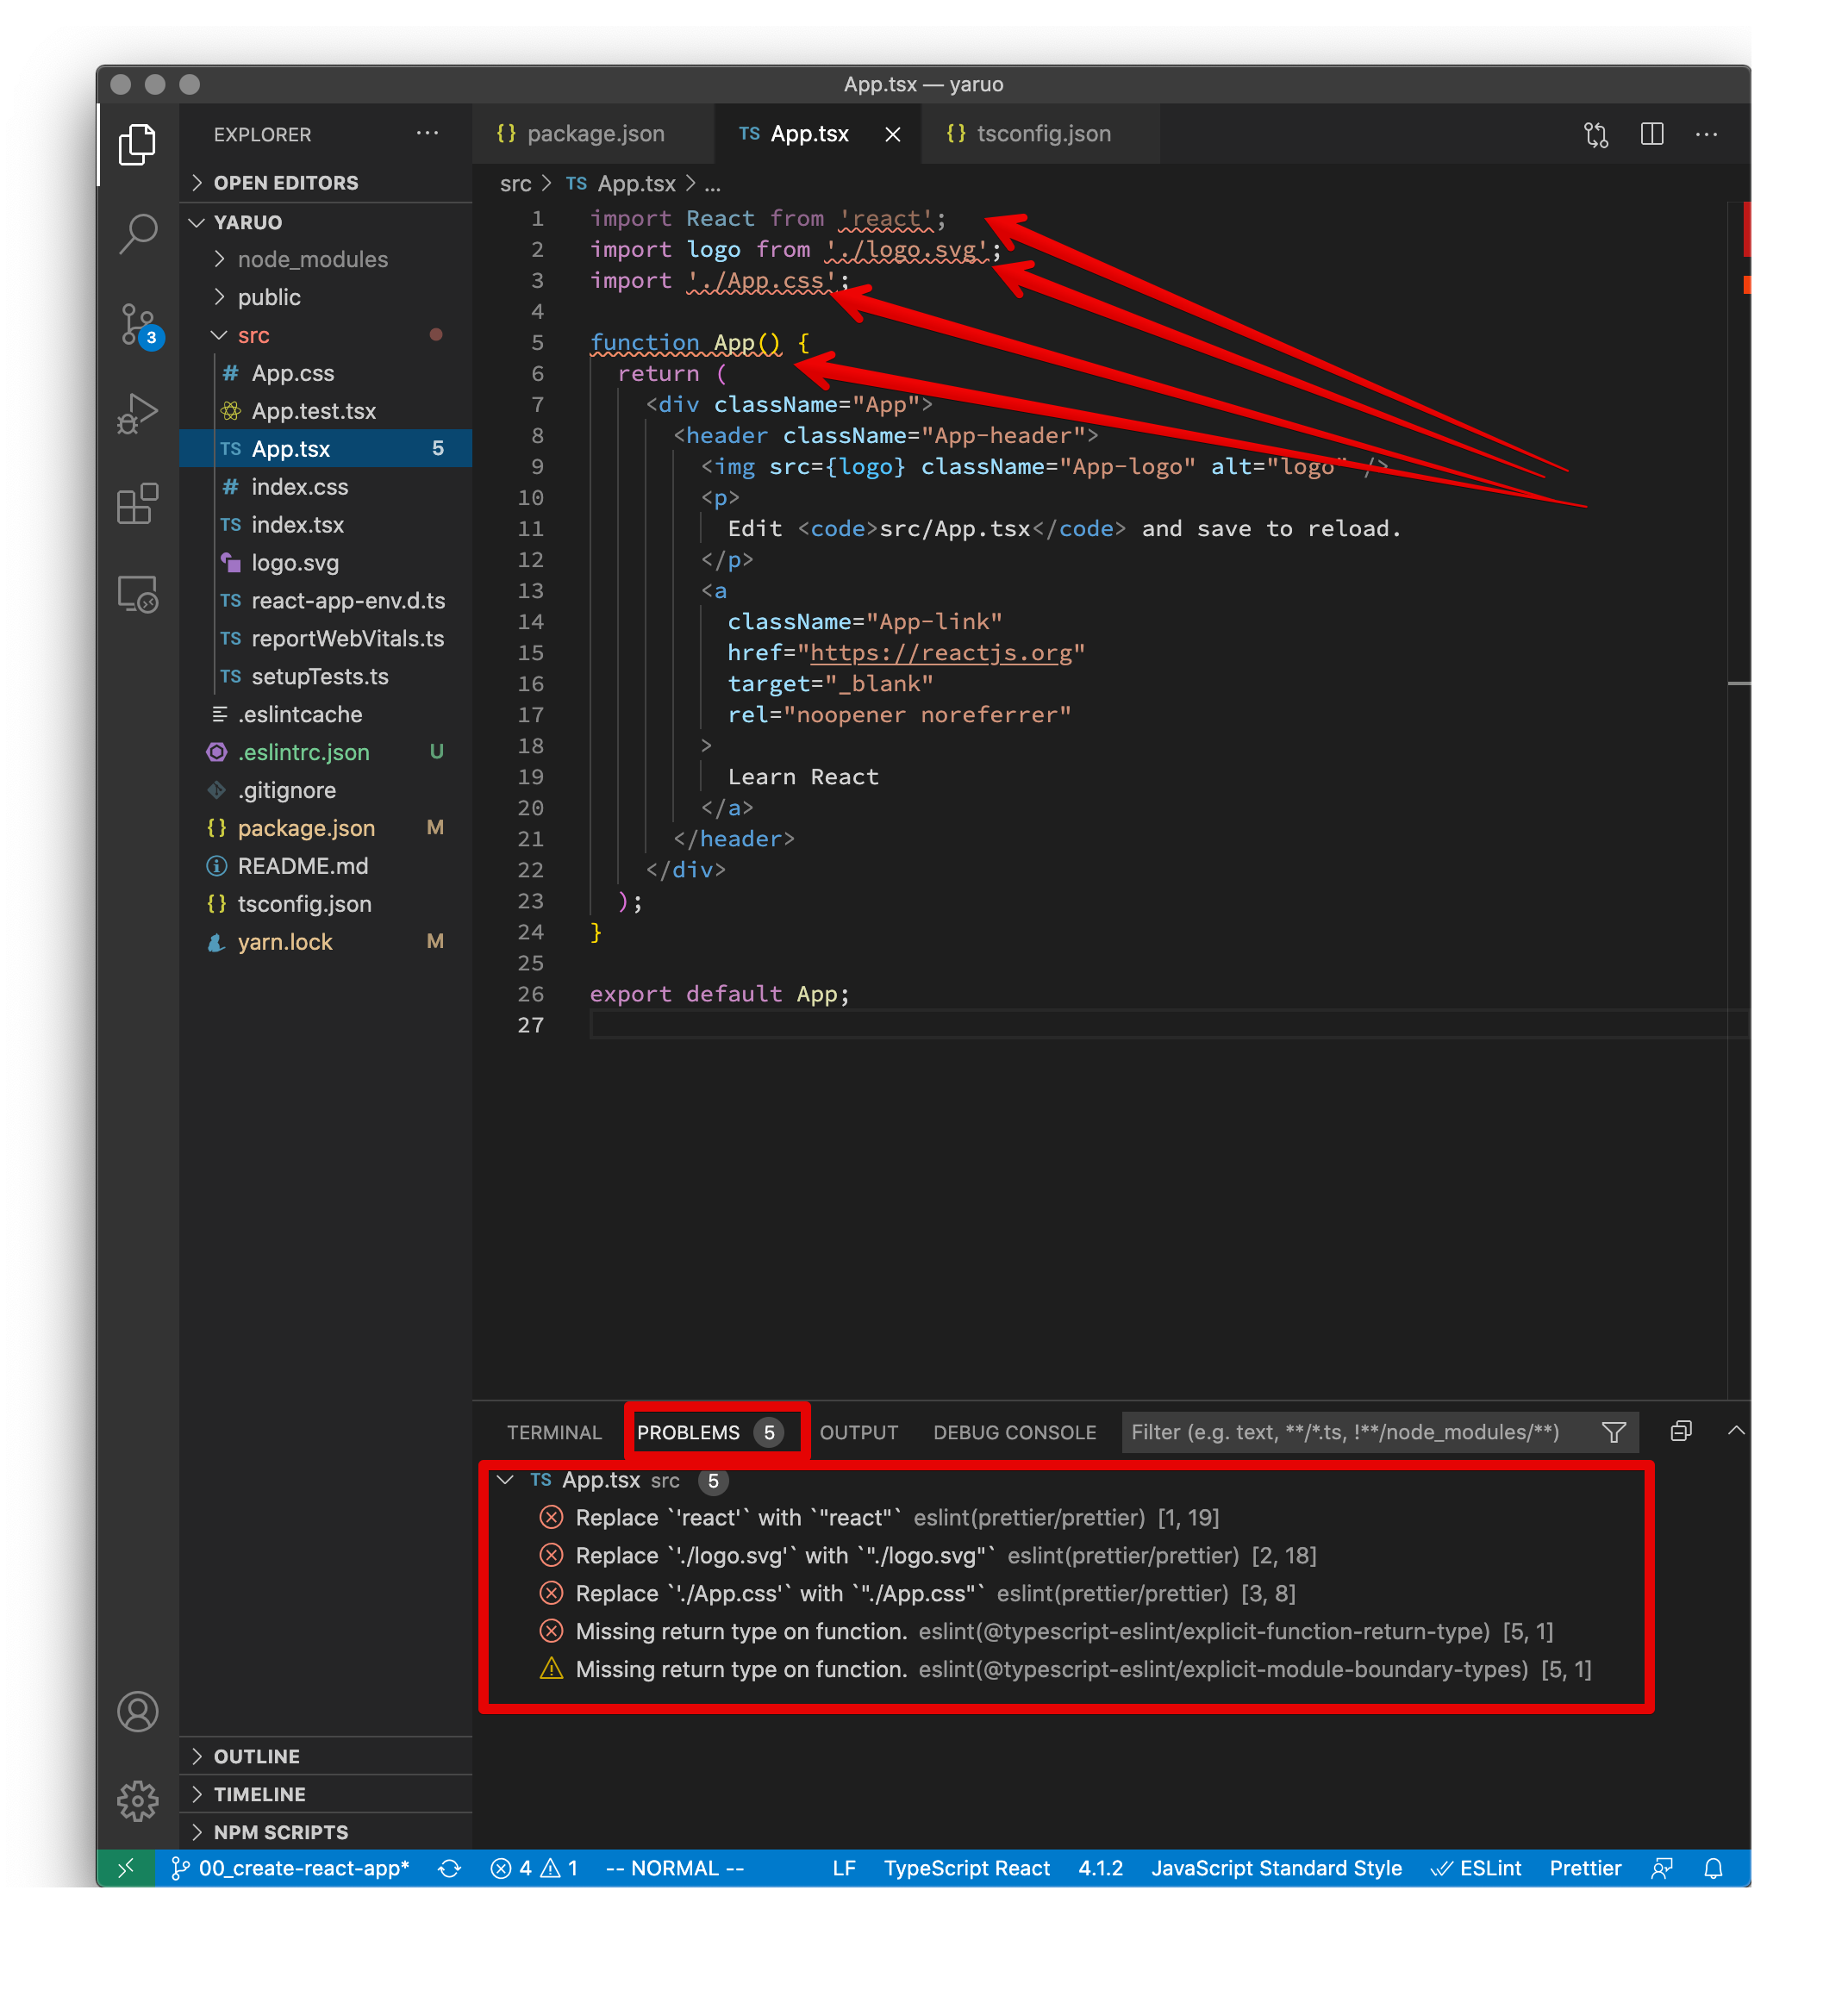
\includegraphics[width=1.0\maxwidth]{./images/02-create-react-app/03_eslint_prettier.png}%
\reviewimagecaption{Eslint、Prettierに怒られてます}
\label{image:02-create-react-app:03_eslint_prettier}
\end{reviewimage}

\section{eslint、prettierの指摘を修正}
\keeplastskip{
  \label{sec:2-4}
  \label{sec-04fix}
  \par\nobreak
}

ESlint、Prettierは指摘するだけではなく、修正案の提示・修正(できるものだけですが・・・)までしてくれます。

VSCode側で設定を行うと、ファイルを保存する度に自動で修正をいれることもできます。

私は、修正を自分のタイミングで行いたいのでVSCode側の設定は行っていません。

もし、VSCode側の設定を行いたい場合には、VSCodeで\\[0pt]
[File] {-}\textgreater{} [Preferences] {-}\textgreater{} [Settings] にて、以下の各項目を検索して設定するか、settings.jsonへ追加してください。

\def\startercodeblockfontsize{}
\begin{starterprogram}[]{VSCodeの設定}\seqsplit{"editor.formatOnSave": true,
"[JavaScript]": \{
  "editor.formatOnSave": false
\},
"[JavaScriptreact]": \{
  "editor.formatOnSave": false
\},
"[typescript]": \{
  "editor.formatOnSave": false
\},
"[typescriptreact]": \{
  "editor.formatOnSave": false
\},
"editor.codeActionsOnSave": \{
    "source.fixAll": true,
    "source.fixAll.eslint": false
\},
"prettier.disableLanguages": ["JavaScript", "JavaScriptreact", "typescript", "typescriptreact"],}\end{starterprogram}

VSCode上で、

\begin{starteritemize}
\item 赤波線で指摘されている
\item 問題タブひ表示sれている
\end{starteritemize}

ものを修正します。

App.tsxの赤波線の上で「コマンドキー(Windowsでは、ctrl) + ピリオド」を押すと、
画面のようにポップアップが表示されます。

\begin{reviewimage}[H]%%04_eslint_prettier_fix
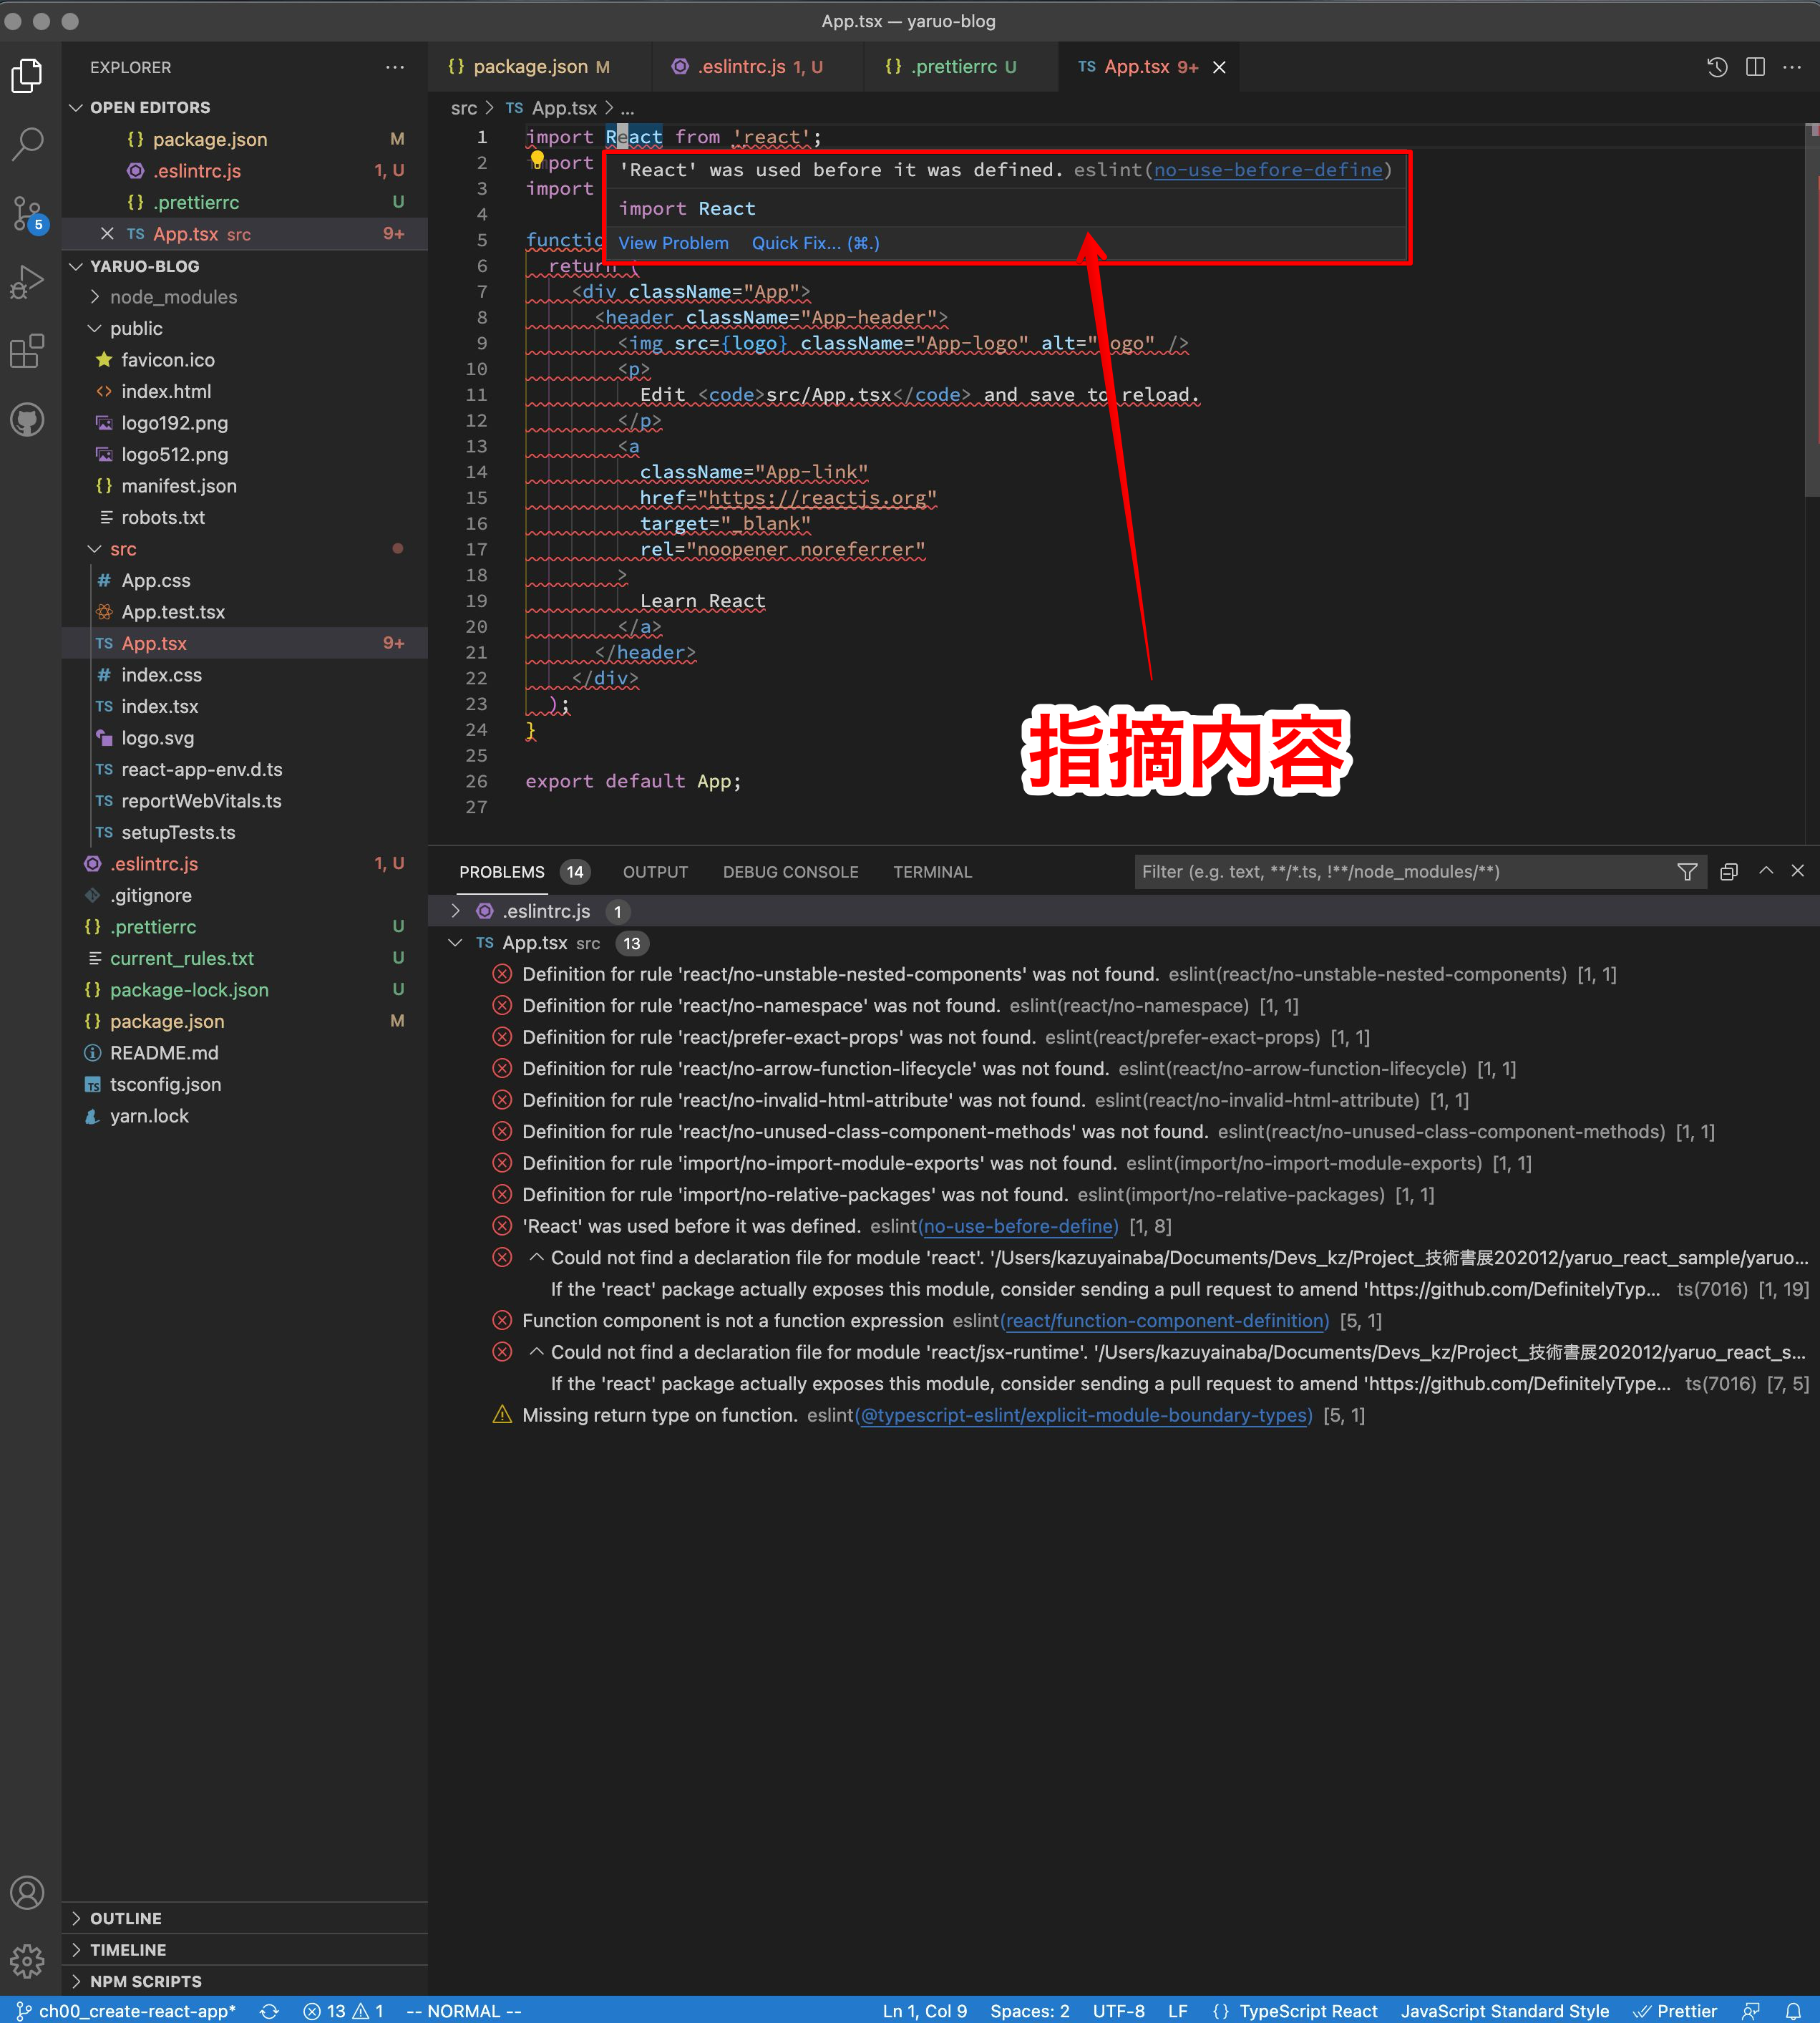
\includegraphics[width=1.0\maxwidth]{./images/02-create-react-app/04_eslint_prettier_fix.png}%
\reviewimagecaption{ポップアップが表示}
\label{image:02-create-react-app:04_eslint_prettier_fix}
\end{reviewimage}

「Fix all auto{-}fixable problems」を選択すると、自動修復可能なものを修正してくれます。

\begin{starternote}[]{}

筆者がVSCodeを日本語化していないのは、エラーメッセージでググる場合を考えてのことです。英語での情報の方が的確なページをみつけやすいと思います。

\end{starternote}

以下のように、修正されたました。

\begin{reviewimage}[H]%%05_eslint_prettier_fixdone
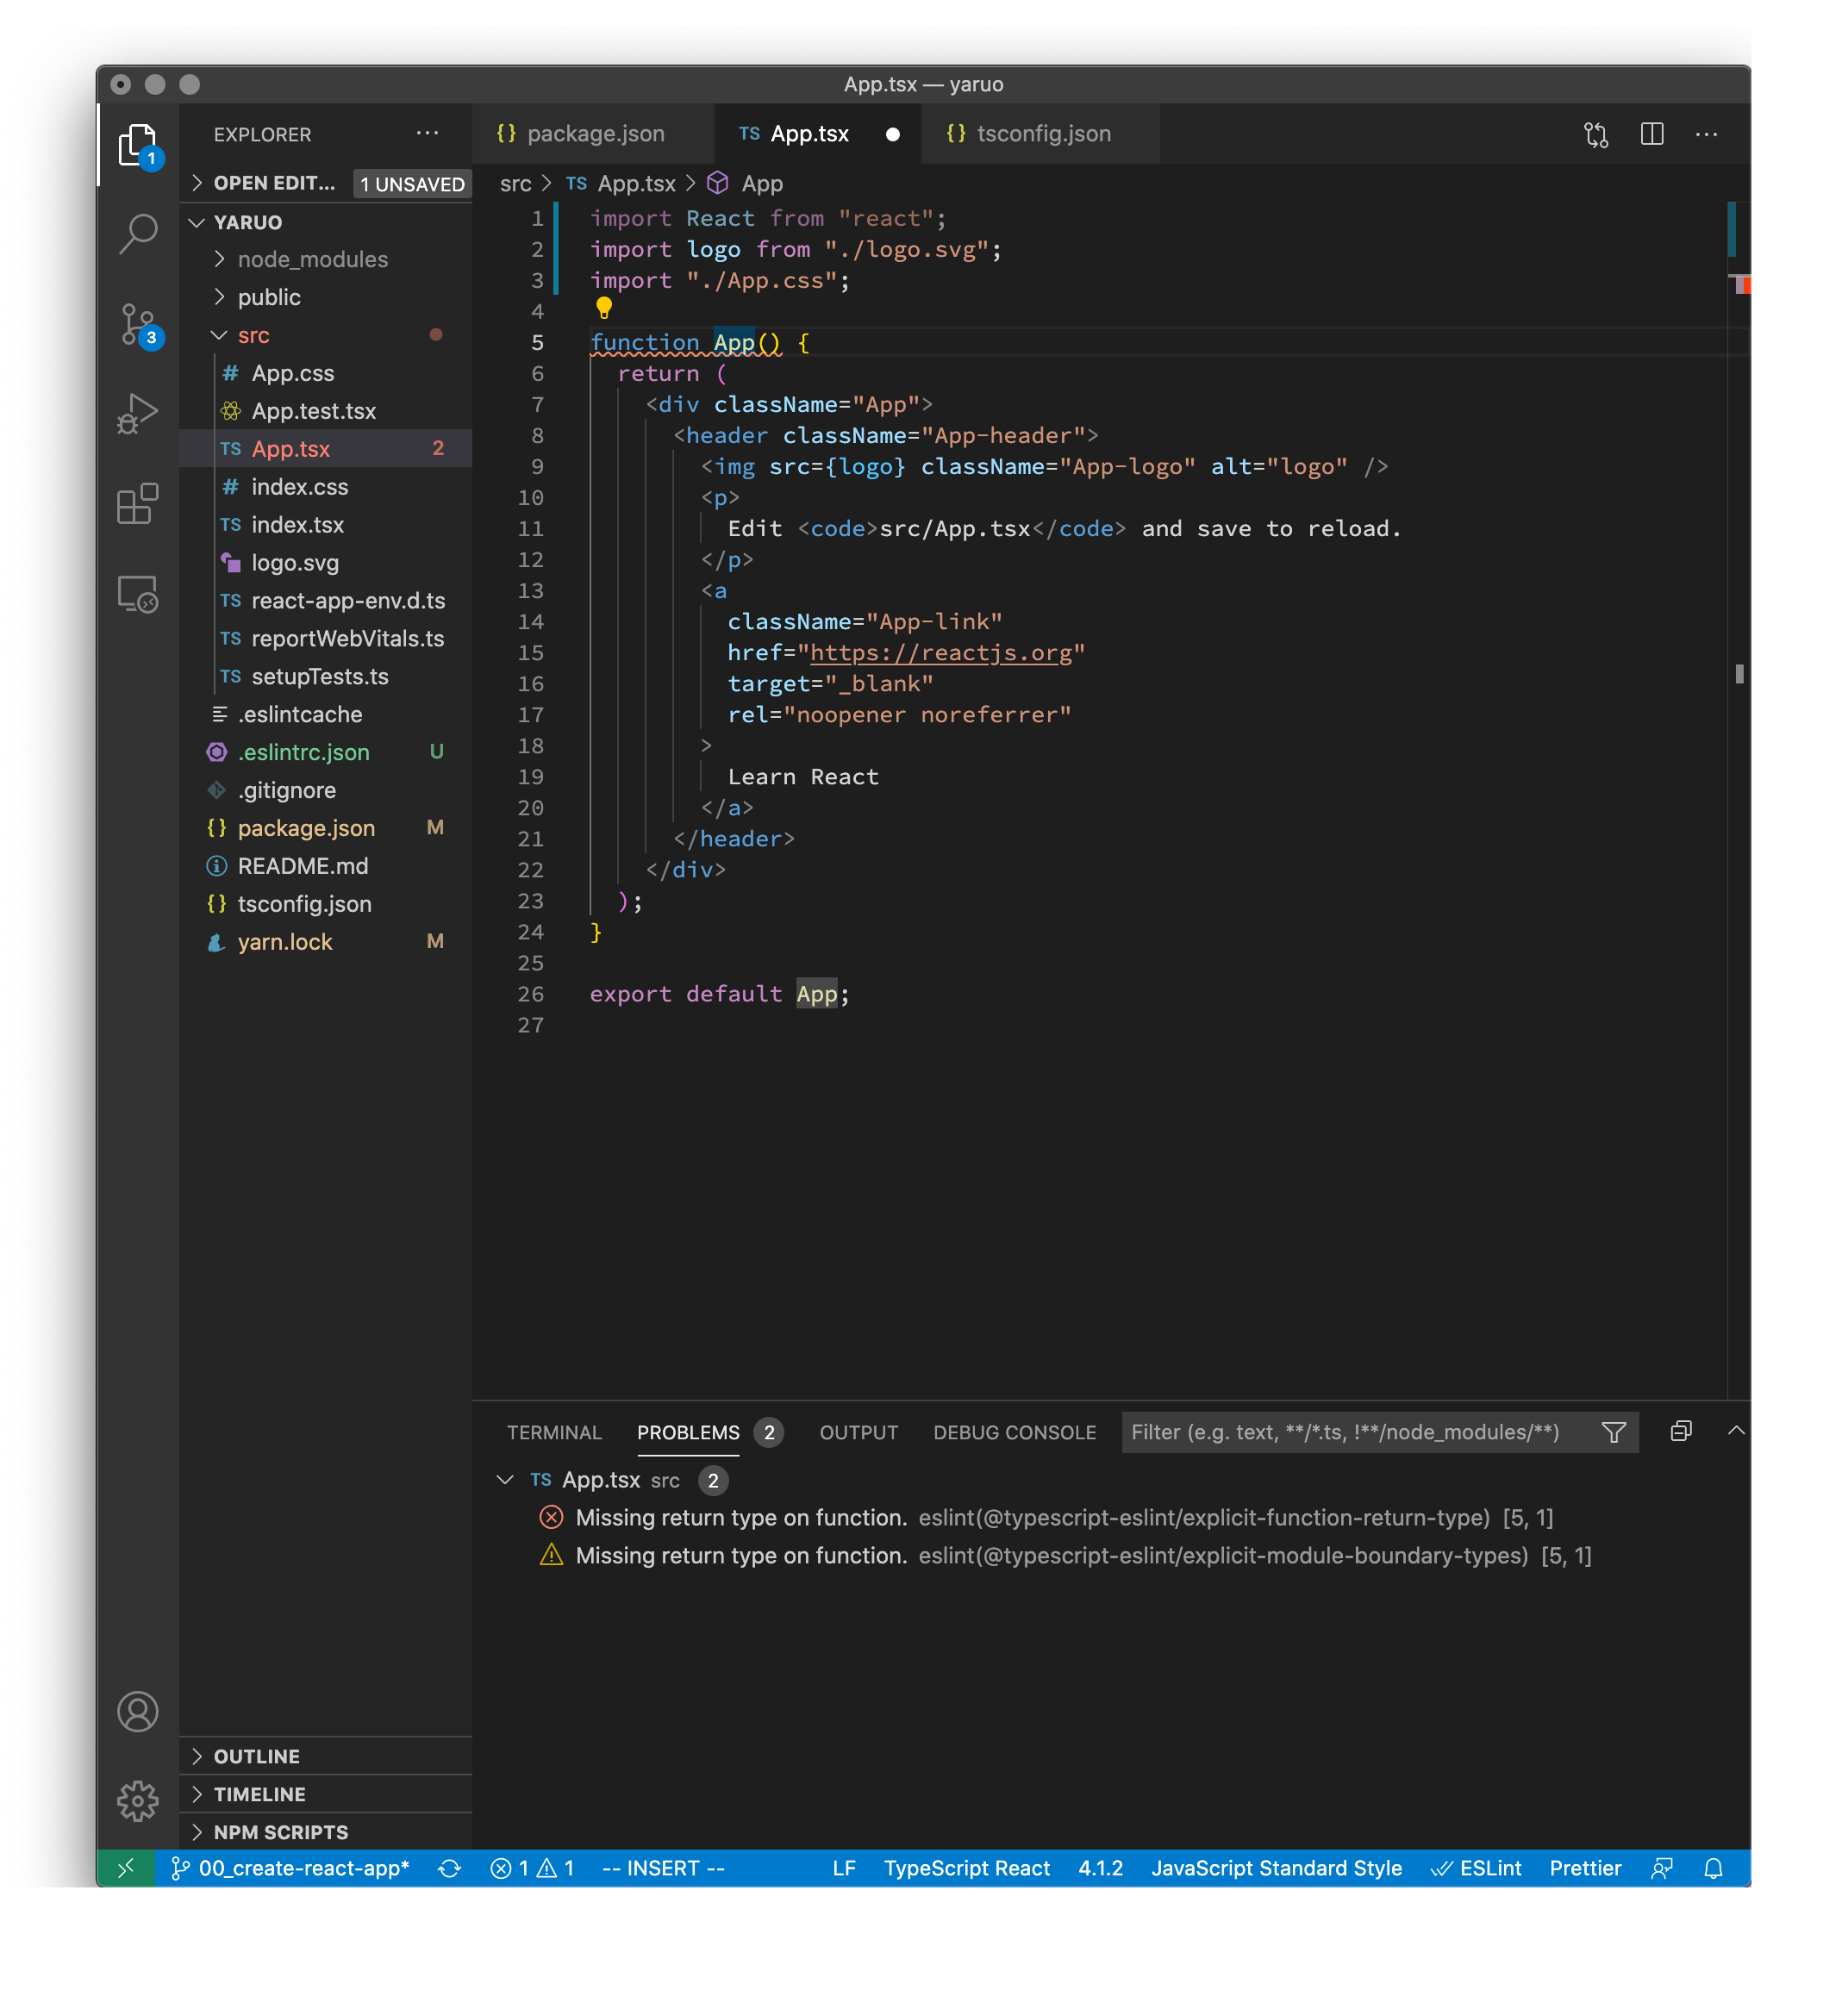
\includegraphics[width=1.0\maxwidth]{./images/02-create-react-app/05_eslint_prettier_fixdone.png}%
\reviewimagecaption{修正後}
\label{image:02-create-react-app:05_eslint_prettier_fixdone}
\end{reviewimage}

自動修正できない問題が残りました。問題点は、このファイルはTypescriptを使用していますので、\\[0pt]
「関数Appの戻り値の型が指定されていない!」\\[0pt]
と言うことです。

ついでに、Arrow関数へ書き換えておきます。

\def\startercodeblockfontsize{}
\begin{starterprogram}[]{App.tsx}\seqsplit{  import React, \{ ReactElement \} from "react";
  import logo from "./logo.svg";
  import "./App.css";

  const App = (): ReactElement =\textgreater{} \{
    return (
      \textless{}div className="App"\textgreater{}}\end{starterprogram}

このように、戻り値の型を指定することで指摘を修正することができました。

\begin{reviewimage}[H]%%06_eslint_prettier_fixdoneAll
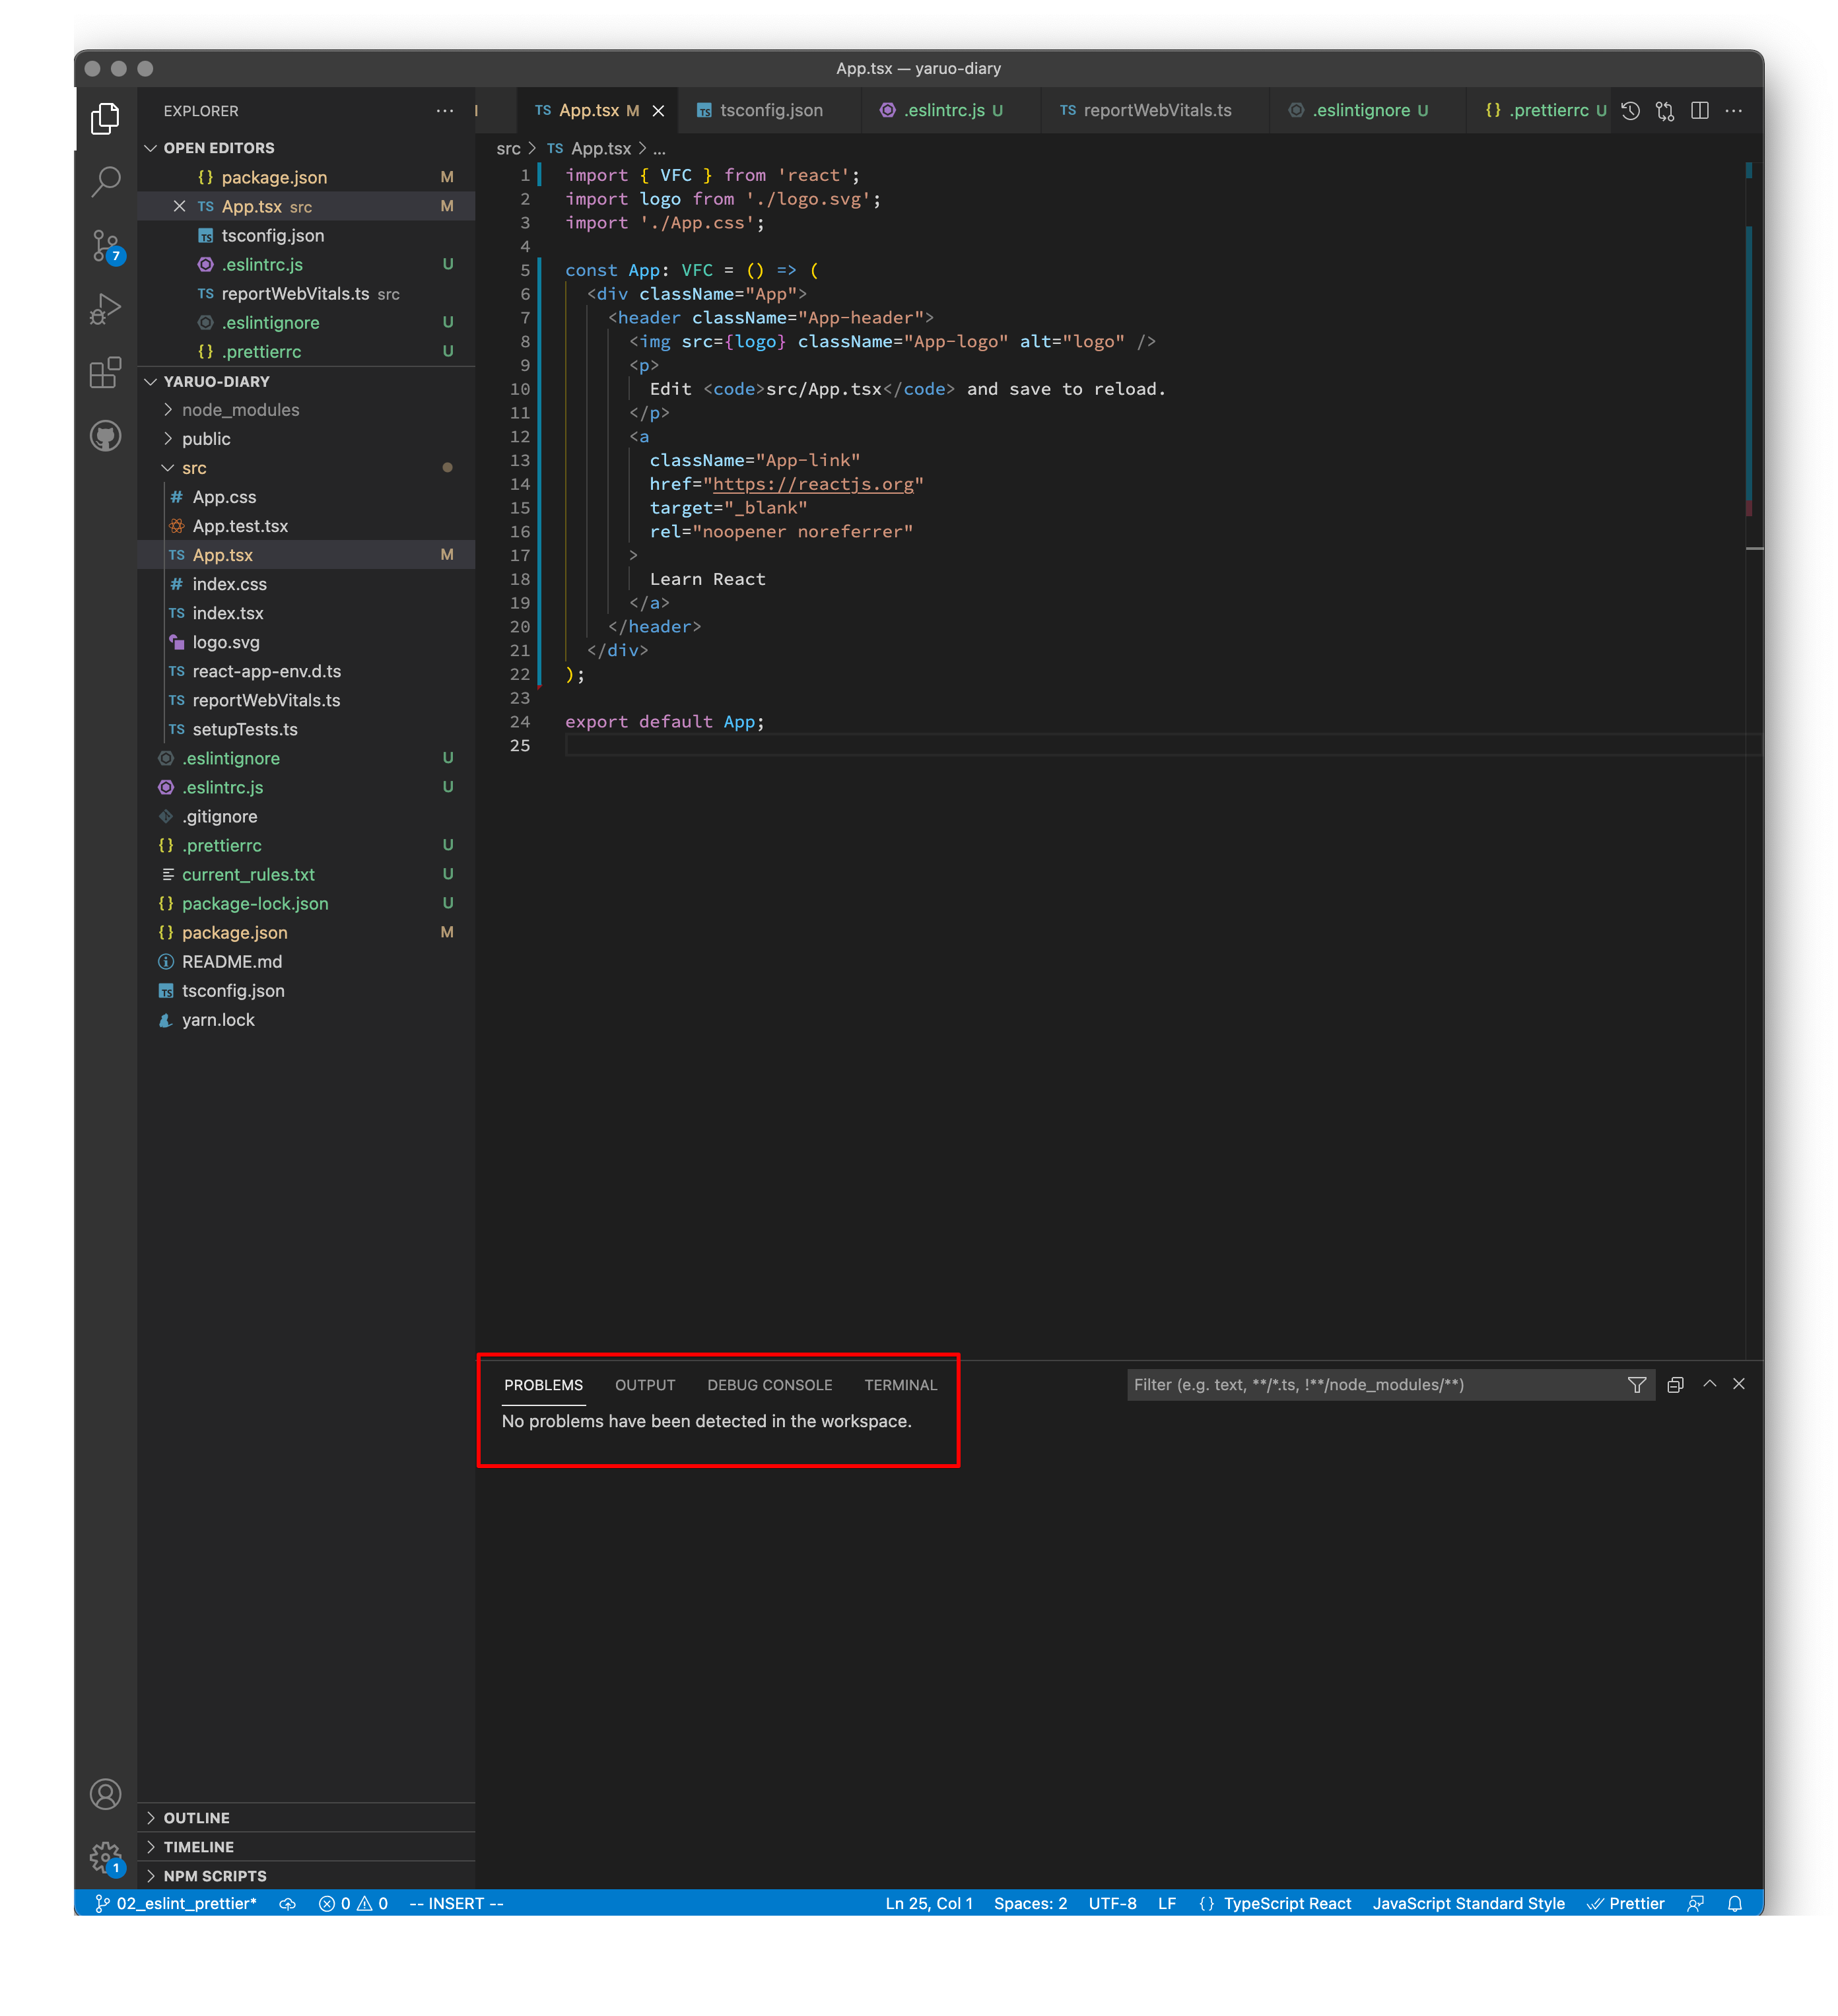
\includegraphics[width=1.0\maxwidth]{./images/02-create-react-app/06_eslint_prettier_fixdoneAll.png}%
\reviewimagecaption{全ての問題の修正完了}
\label{image:02-create-react-app:06_eslint_prettier_fixdoneAll}
\end{reviewimage}

\section{第2章のまとめ}
\keeplastskip{
  \label{sec:2-5}
  \label{sec-chap02review}
  \par\nobreak
}

Reactを使用したアプリケーションは、スタートアップ用のアプリケーションがコマンド一発でインストールできます。

より良いコーディングをするためにも、Eslint、Prettierを導入しましょう。

\begin{starternote}[]{}

ここまでの内容は、github上で、以下のコマンドでクローンできます。

\def\startercodeblockfontsize{}
\begin{starterterminal}[]{github}\seqsplit{  \textdollar{} \textgreater{} git clone {-}b 01\textunderscore{}eslint\textunderscore{}prettier https://github.com/tmkkz/yaruo.git}\end{starterterminal}
\end{starternote}
